\section{Budget Awareness}

 

\begin{figure}[h] 
    \centering
    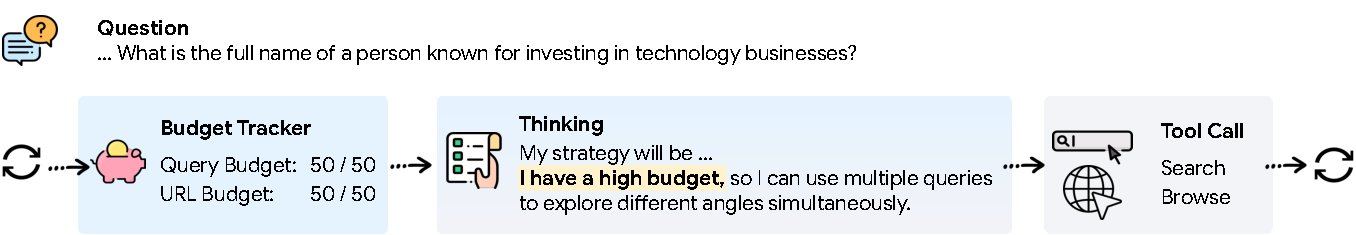
\includegraphics[width=\textwidth]{assets/figs/bt_fig.pdf} 
    \caption{At each interaction round, the agent is provided with its current and remaining budget through the budget tracker before generating the next thinking step and the tool call actions.}
    \label{fig:framework}
\end{figure}

\subsection{Budget Tracker}

Each tool invocation introduces non-negligible costs in context and computation. We hypothesize that providing explicit budget signals enables the model to internalize resource constraints and adapt its strategy without requiring additional training.

We introduce \textbf{Budget Tracker}, a lightweight, plug-and-play module that surfaces real-time budget states inside the agent’s reasoning loop.
In the beginning iteration, the tracker provides a brief policy guideline describing the budget regimes and corresponding tool-use recommendations~(see Appendix~\ref{app:prompts}).
At each subsequent iteration, this tracker appends a budget status block showing the remaining and used budgets for each available tool:



\begin{tcolorbox}[
  enhanced,
  breakable,
  colback=white,
  colframe=black!10!white, 
  coltitle=black!80!white, 
  title={Budget Tracker},
  % fonttitle=\large\bfseries,
]
\small
<budget>

Tool$_{1}$ Budget Used: \#\#, Tool$_{1}$ Budget Remaining: \#\#

Tool$_{2}$ Budget Used: \#\#, Tool$_{2}$ Budget Remaining: \#\#

Make the best use of the available resources.

</budget>
\end{tcolorbox}



Despite its simplicity, Budget Tracker operates purely at the prompt level and makes the agent explicitly aware of its resource consumption and remaining budget, enabling it to condition subsequent reasoning steps on the updated resource state.



\subsection{Scaling with Budget Awareness} 
To better understand how agent behaviors scale under different budget constraints, we study two mainstream test-time scaling paradigms: \emph{sequential scaling} and \emph{parallel scaling}. 

In \textit{sequential scaling}, we adopt the budget-forcing strategy~\citep{DBLP:journals/corr/abs-2501-19393} by appending the following message when the agent proposes an answer: ``Wait, you still have remaining tool budget, use more search and browse tools to explore different information sources before concluding.''
This encourages the model to reevaluate its reasoning and make better use of its available tool calls.
In \textit{parallel scaling}, we fix the per-run budget and conduct multiple independent runs in parallel.
We report Majority Vote, Best-of-N and Pass@N results, following common test-time scaling practice~\citep{DBLP:journals/corr/abs-2504-12516}. More details can be found in Appendix~\ref{app:pass@n}.



\subsection{Results and Analysis}

We evaluate Budget Tracker on three information-seeking QA datasets requiring external search: BrowseComp~\citep{DBLP:journals/corr/abs-2504-12516}, BrowseComp-ZH~\citep{DBLP:journals/corr/abs-2504-19314} and HLE-Search~\citep{DBLP:journals/corr/abs-2501-14249, DBLP:journals/corr/abs-2507-16075}. Dataset details and full experimental setup are provided in Section~\ref{sec:exp}.
Building on the ReAct framework, we incorporate the Budget Tracker immediately after each tool response to inform the agent of its remaining budget. Each tool is assigned a budget of 100, and the reasoning process stops when any budget is exhausted or the agent reaches a final answer.

\begin{table}[ht]
\centering
% \small
\caption{Effect of Budget Tracker on tool-use behavior and performance. 
Adding the tracker consistently improves answer accuracy  across models and datasets. Results are averaged across three runs.}\label{tab:react_bab}
\begin{tabular}{llrrr}
\toprule
\textbf{Model} & \textbf{Method} & \textbf{BrowseComp} & \textbf{BrowseComp-ZH} & \textbf{HLE-Search} \\
\midrule
\multirow{2}{*}{Gemini-2.5-Pro} 
& ReAct & 12.6 & 31.5 & 20.5\\
& + Budget Tracker & \textbf{14.6}  & \textbf{32.9} & \textbf{21.8}\\
\midrule
\multirow{2}{*}{Gemini-2.5-Flash} 
& ReAct & 9.7 & 26.5 & 14.7\\
& + Budget Tracker & \textbf{10.7}  & \textbf{28.7} & \textbf{17.3} \\
\midrule
\multirow{2}{*}{Claude-Sonnet-4} 
& ReAct & 12.2 & 29.1 & 20.5 \\
& + Budget Tracker & \textbf{14.0}  & \textbf{31.1} & \textbf{23.0} \\
\bottomrule
\end{tabular}
\end{table}

\textbf{Budget Tracker enables higher performance under the same budget.}
Table~\ref{tab:react_bab} compares ReAct with and without the Budget Tracker under identical budget limits. Across different models, adding the tracker consistently improves accuracy on all the datasets.  This demonstrates that making budget signals explicit encourages more strategic and positive agent tool-use behavior.



\begin{table}[t]
\centering
\caption{Performance and resource consumption comparison under different budgets using Gemini-2.5-Pro. With 10$\times$ less budget (10 vs.\ 100), Budget Tracker achieves comparable accuracy while requiring fewer tool calls and lower total cost, highlighting the benefits of explicit budget awareness.}
\label{tab:react_less_cost}
\begin{tabular}{lrrrrr}
\toprule
\multirow{2}{*}{\textbf{Methods}} & 
\multirow{2}{*}{\textbf{Budget}} & 
\multirow{2}{*}{\textbf{Acc (\%)}} &
\multicolumn{3}{c}{\textbf{Consumed resources}} \\ 
\cmidrule(lr){4-6}
 &  &  & \textbf{\# search} & \textbf{\# browse} & \textbf{Unified cost (¢)} \\
\midrule
\multirow{3}{*}{ReAct} 
 & 10  & 10.3 & 7.87  & 0.60 & 5.2 \\
 & 30  & 10.5 & 13.77 & 1.33 & 8.0 \\
 & 100 & 12.6 & 14.24 & 1.36 & 9.9 \\
\midrule
\textbf{ReAct + Budget Tracker} & 10 & \textbf{12.8} & 8.48 & 1.09 & 6.8 \\
\bottomrule
\end{tabular}
\end{table}

\begin{wrapfigure}{r}{0.5\textwidth}
    \centering
    % \vspace{-10pt} 
    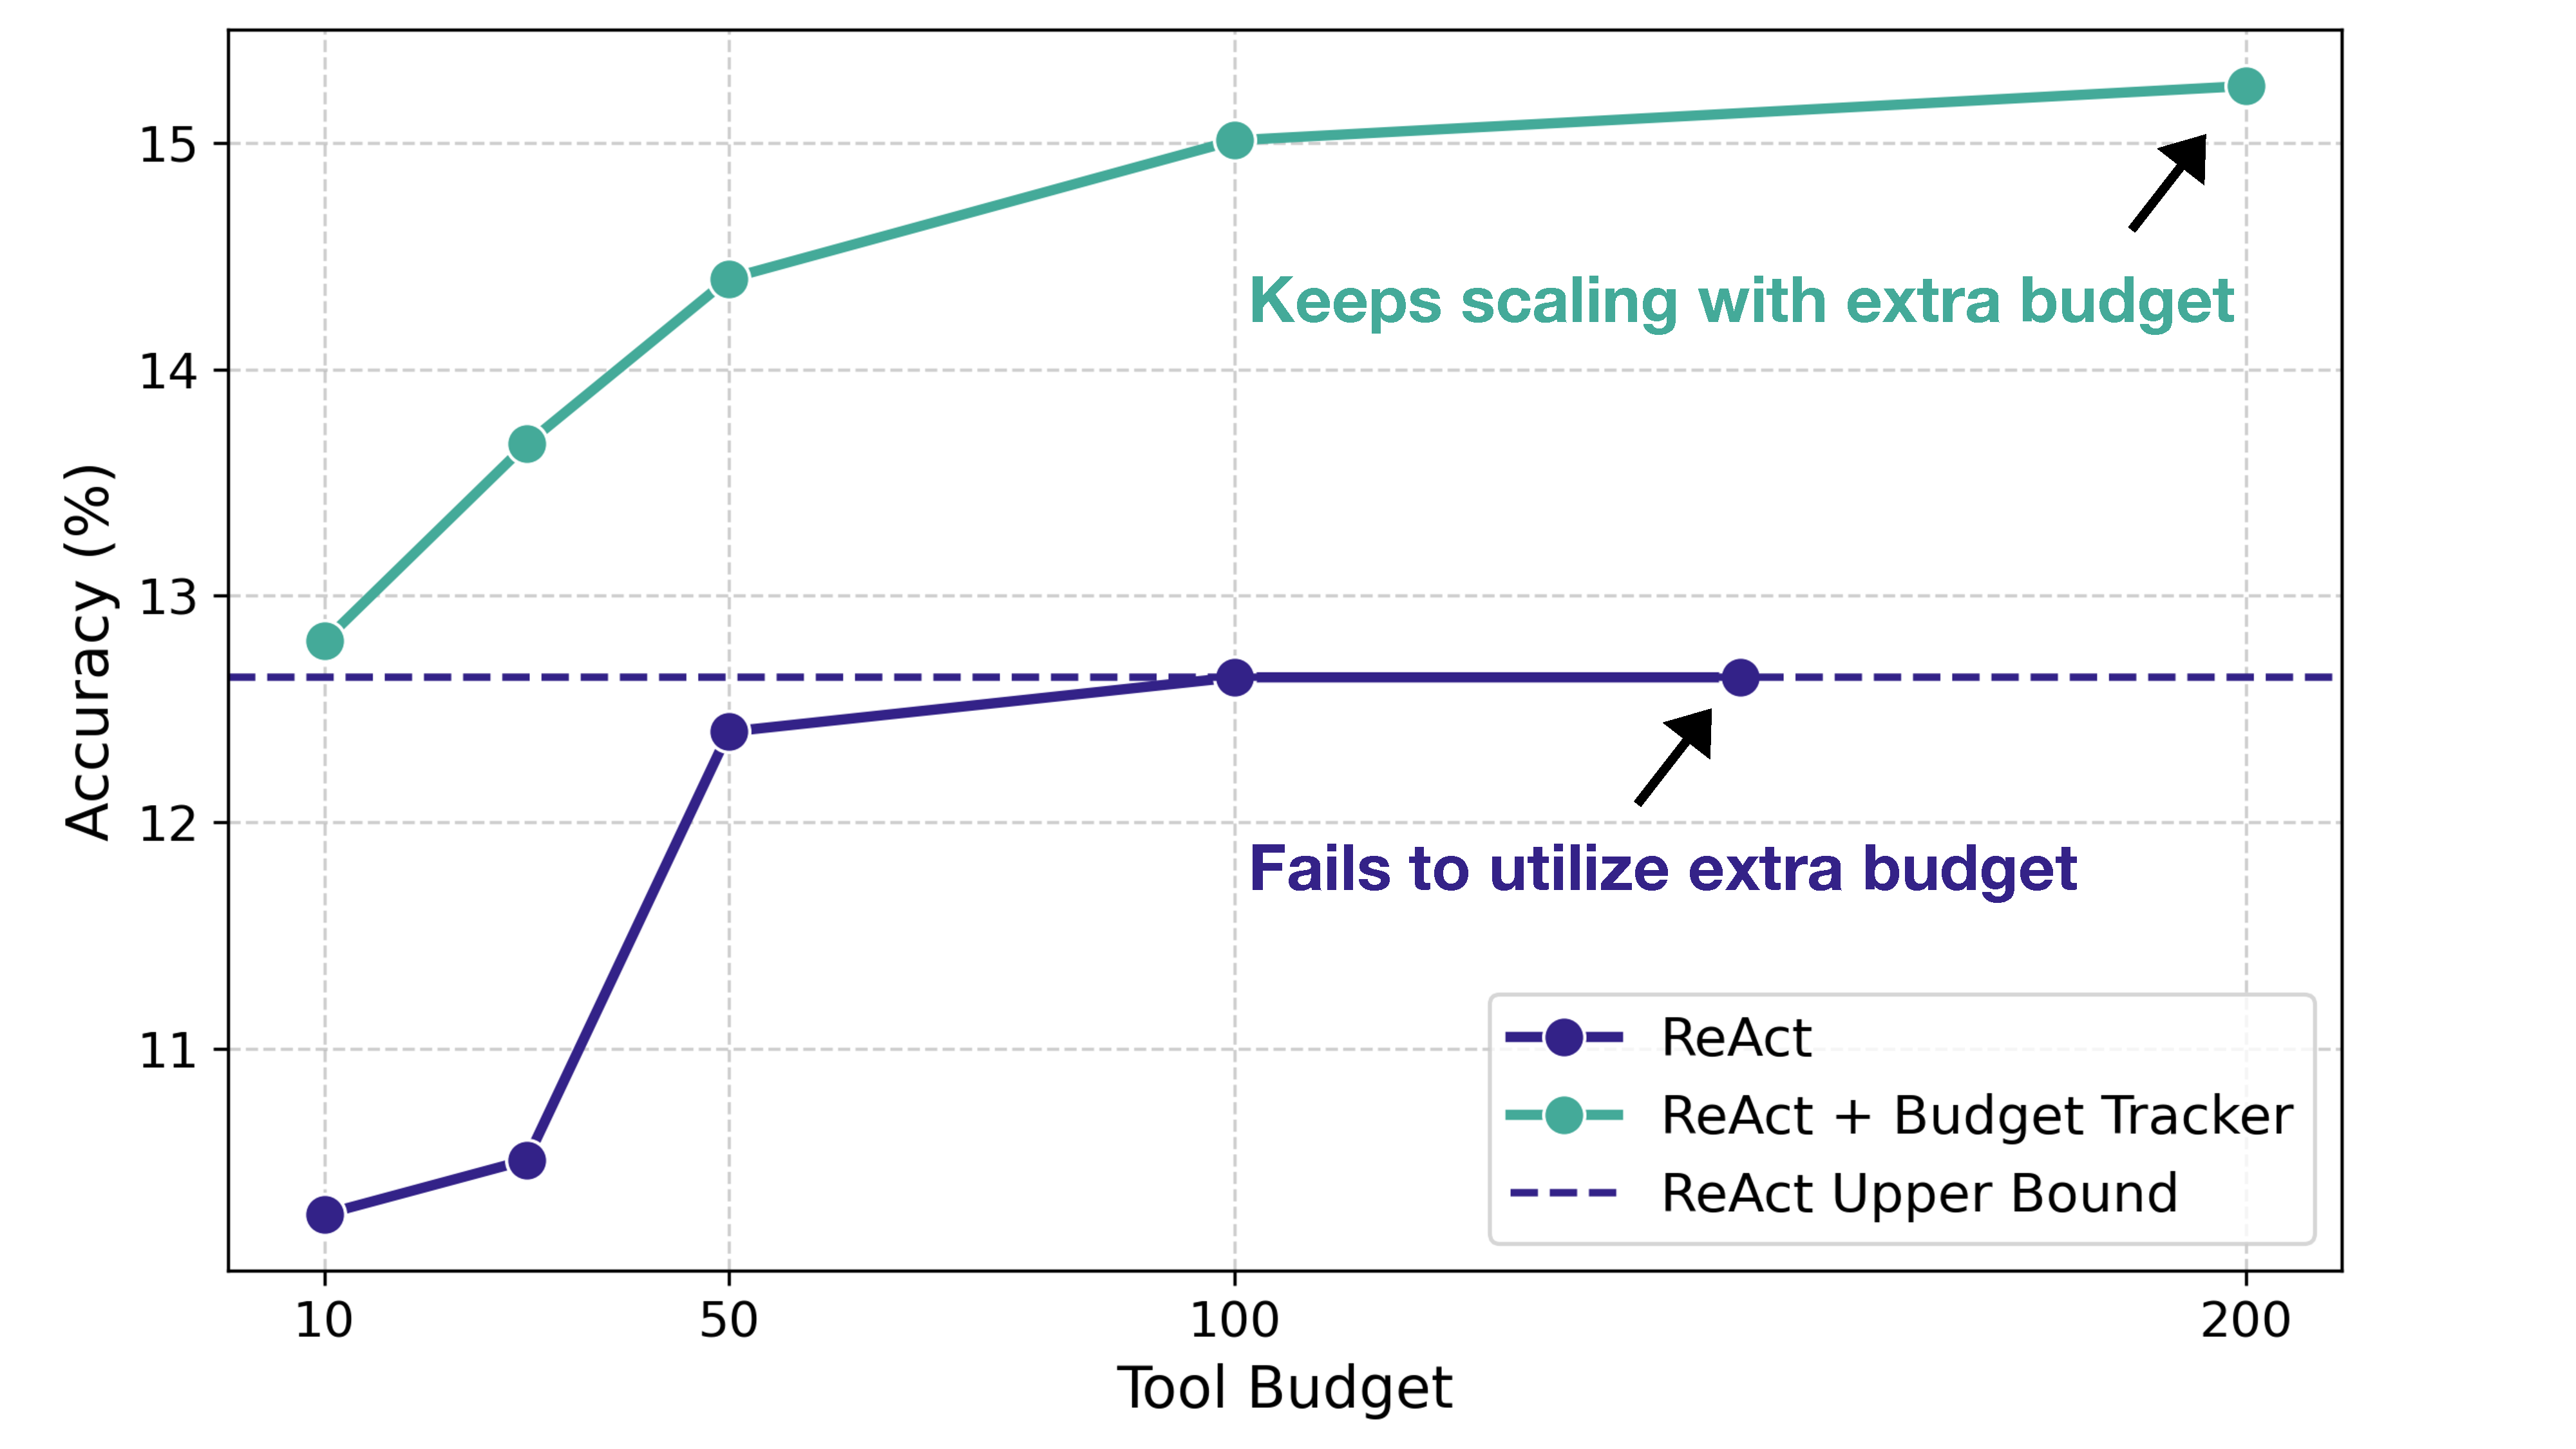
\includegraphics[width=0.5\textwidth]{assets/figs/bt_no_cg.pdf}
    \caption{ReAct saturates and fails to utilize additional tool budget, reaching a performance ceiling. In contrast, ReAct + Budget Tracker continues to scale effectively with larger budgets, achieving consistent accuracy improvements.}
    \label{fig:bt_no_cg}
    \vspace{-5pt} 
\end{wrapfigure}


\textbf{Budget Tracker achieves lower resource usage and cost under similar accuracy.}
In Table~\ref{tab:react_less_cost}, the consumed resources report the average number of search and browse tool calls, as well as the unified cost combining tool usage and token consumption per question.
Increasing the tool-use budget in ReAct improves performance but also raises both tool call frequency and total cost. In contrast, Budget Tracker achieves comparable accuracy with less budget (10 vs.\ 100), while using 40.4\% fewer search calls, 21.4\% fewer browse calls, and reducing overall cost by 31.3\%. This demonstrates that explicit budget awareness enables more efficient tool use without sacrificing accuracy.




\textbf{Budget Tracker facilitates continued scaling through effective resource utilization by simply adding budget awareness.} Figure~\ref{fig:bt_no_cg} illustrates Gemini-2.5-Pro's performance on BrowseComp as tool budget increases. Lacking budget awareness, the standard ReAct baseline saturates at a budget of 100. Beyond this point, it fails to utilize any additionally allocated budget, even though the context window is not filled up.
This ceiling occurs because the agent's reasoning process terminates prematurely: it either believes it has found a sufficient answer or concludes it is stuck and gives up, unaware of the unused resources.
In contrast, Budget Tracker explicitly informs the model of its remaining resources, enabling it to leverage larger budgets and continue scaling its performance.



\subsection{Analysis on Test-time Scaling Strategies}

Across different test-time scaling strategies, \textbf{Budget Tracker consistently pushes the Pareto frontier and demonstrates robust effectiveness.}
Sequential scaling encourages the agent to issue more tool calls by prompting it to continue reasoning and exploring additional information sources. The prompting stops once the agent refuses to invoke any tools for five iterations. As shown in Figure~\ref{fig:bt_seq_pro}, while this strategy enables ReAct to further improve accuracy, it eventually encounters a performance ceiling, where the agent confidently concludes that no further tool calls are necessary. In contrast, Budget Tracker achieves a consistently better scaling curve and sustains performance gains beyond ReAct's plateau. Furthermore, it advances the Pareto frontier of the cost--performance curve, demonstrating not only more effective performance scaling but also more efficient tool utilization.

\begin{figure}[t]
    \centering
    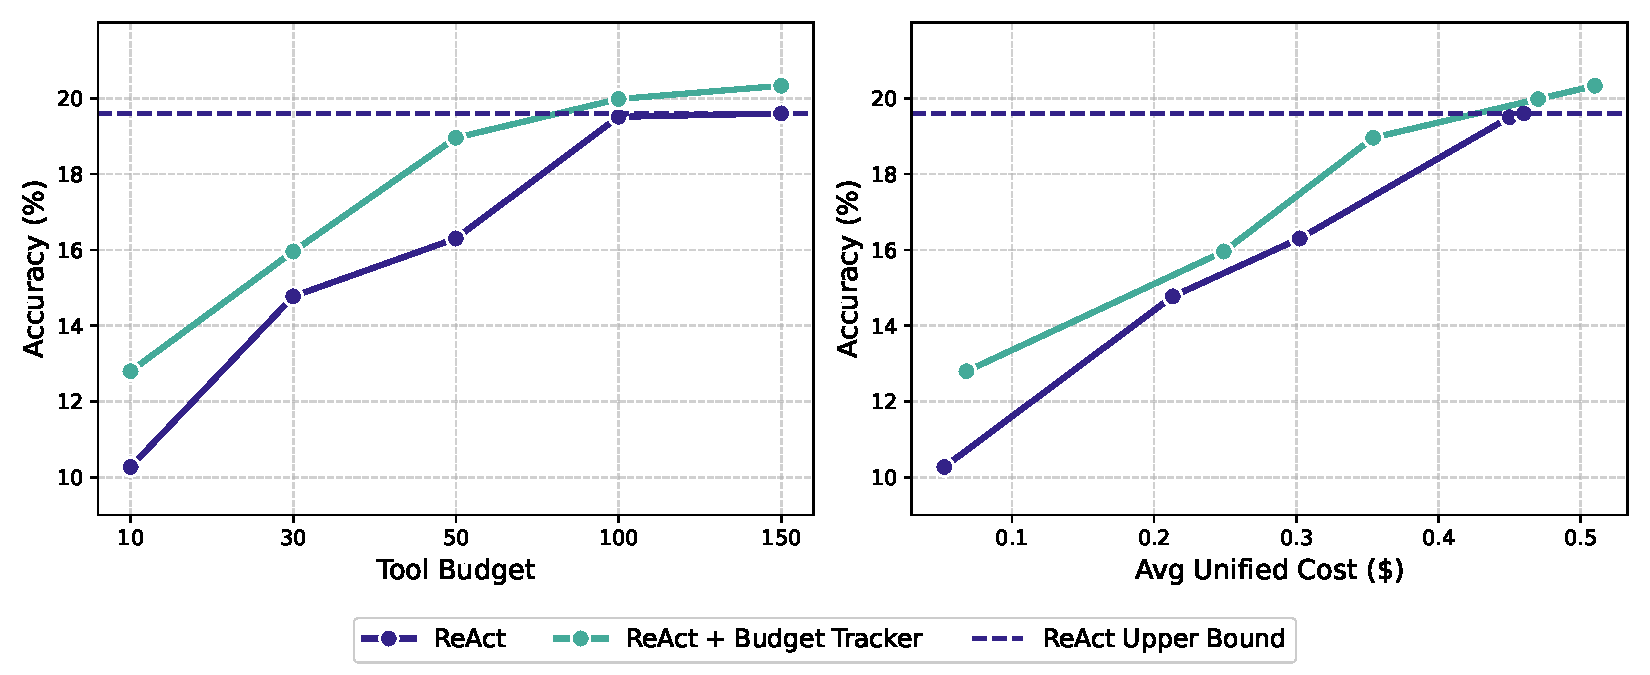
\includegraphics[width=0.9\linewidth]{assets/figs/bt_seq_pro.pdf}
    \caption{Comparison of Budget Tracker and ReAct in sequential scaling using Gemini-2.5-Pro. With explicit budget awareness, Budget Tracker consistently improves upon ReAct at equal budgets. ReAct plateaus early as it cannot utilize extra resources, while Budget Tracker adapts its spending to gain further improvements and extend the cost-performance frontier.
    }
    \label{fig:bt_seq_pro}
\end{figure}



For parallel scaling, we set a fixed budget of 50 per run for Gemini-2.5-Pro, as empirical observations indicate that only 0.8\% of the data in BrowseComp requires exceeding this limit (see details in Appendix~\ref{app:usage_breakdown}). In Figure~\ref{fig:bt_parallel_all}, we use identical sample sizes for both settings and report Majority Vote and Best-of-N results (Pass@N results are provided in Appendix~\ref{app:pass@n}). On the right, the figure illustrates the cost--performance scaling, where Budget Tracker consistently yields a superior curve.




\begin{figure}[t]
    \centering
    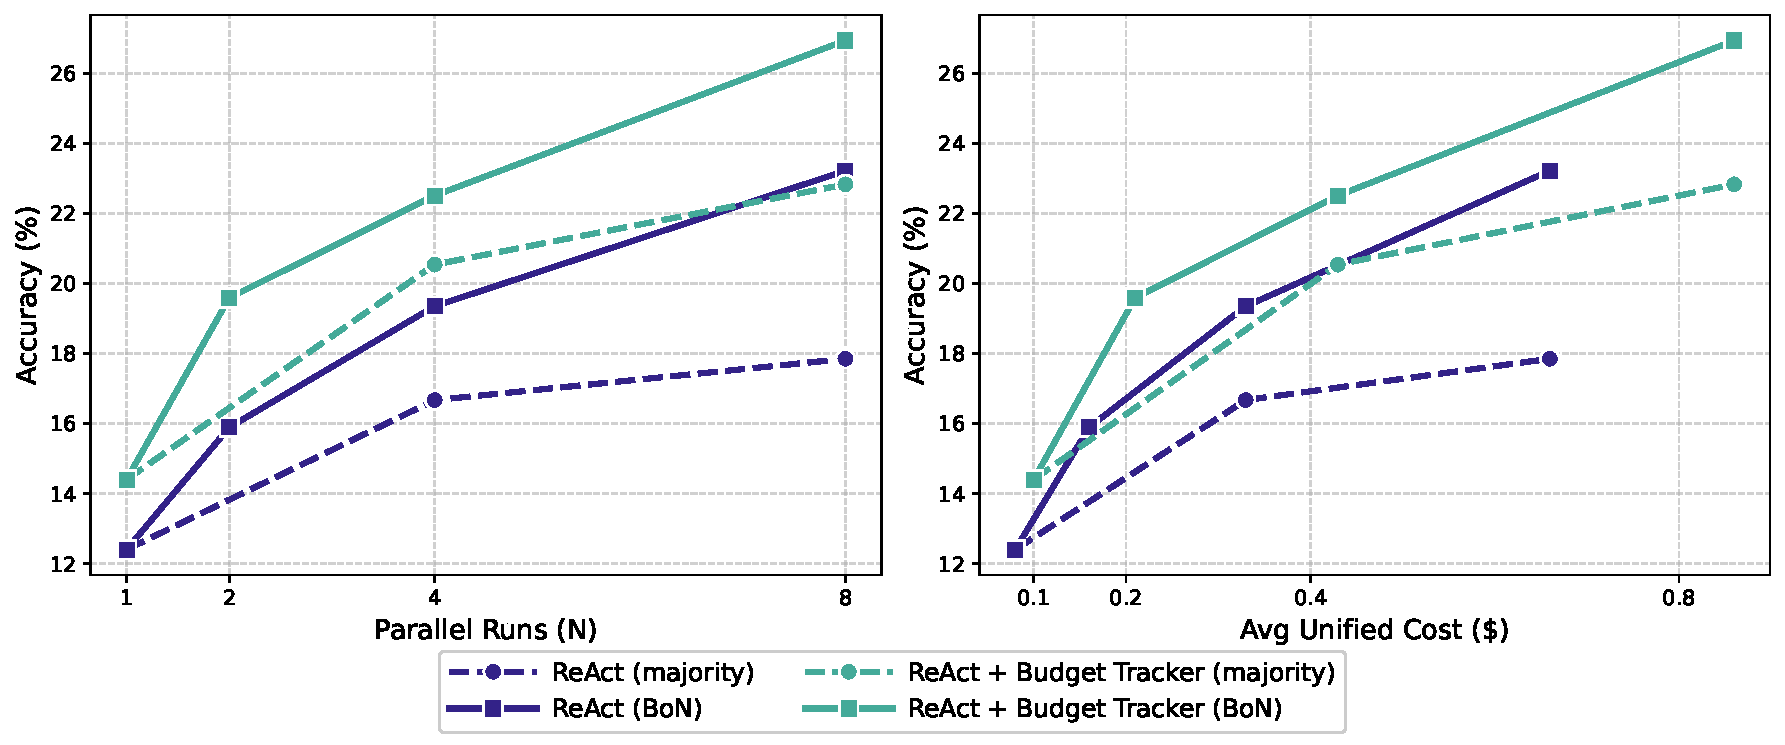
\includegraphics[width=0.85\linewidth]{assets/figs/bt_parallel_combined_bon.pdf}
    \caption{Comparison of Budget Tracker and ReAct in parallel scaling using Gemini-2.5-Pro. 
The left subfigure shows accuracy scaling with increasing parallel runs, 
while the right subfigure illustrates the corresponding cost–performance trend.
    }
    \label{fig:bt_parallel_all}
\end{figure}
